\documentclass[10pt]{article}
\usepackage[polish]{babel}
\usepackage[utf8]{inputenc}
\usepackage[T1]{fontenc}
\usepackage{amsmath}
\usepackage{amsfonts}
\usepackage{amssymb}
\usepackage[version=4]{mhchem}
\usepackage{stmaryrd}
\usepackage{graphicx}
\usepackage[export]{adjustbox}
\graphicspath{ {./images/} }

\title{GIMNAZJUM }

\author{}
\date{}


\begin{document}
\maketitle
\begin{enumerate}
  \item Odcinek \(A B\) ślizga się po ramionach kąta prostego w ten sposób, że punkt \(A\) należy do jednego ramienia, a punkt \(B\) do drugiego. Jaki kształt będzie miała droga, którą przebędzie środek odcinka \(A B\). Odpowiedź uzasadnij.
  \item Czworokąt wypukły podzielono na cztery części łącząc środki jego boków jak na rysunku. Wykaż, że suma pól części zacienionych jest równa sumie pól części niezacienionych.
  \item Wykaż, że w trójkącie \(A B C\) dwusieczna kąta \(A C B\) i symetralna\\
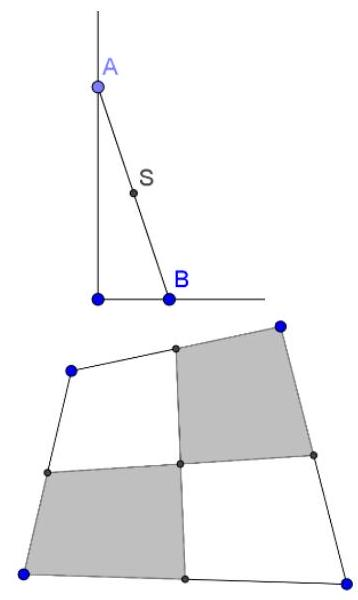
\includegraphics[max width=\textwidth, center]{2024_11_21_9bcf201a4fb59f89a03bg-1(1)}\\
boku \(A B\) przecinają się na okręgu opisanym na tym trójkącie.
\end{enumerate}

\section*{LICEUM}
\begin{enumerate}
  \item Trójkąt prostokątny \(A B C\) ślizga się po ramionach kąta prostego w ten sposób, że punkt \(A\) należy do jednego ramienia, a punkt \(B\) do drugiego. Jaki kształt będzie miała droga, którą przebędzie wierzchołek kąta prostego \(C\). Odpowiedź uzasadnij.\\
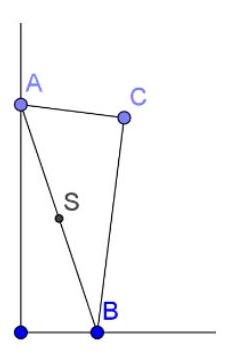
\includegraphics[max width=\textwidth, center]{2024_11_21_9bcf201a4fb59f89a03bg-1}
  \item Czworokąt wypukły podzielono na dziewięć części dzieląc każdy bok na trzy równe części i łącząc punkty podziału jak na rysunku. Wykaż, że suma pól części czerwonych jest równa sumie pól części niebieskich. Uwaga! Nie jest oczywiste, że wszystkie odcinki łączące punkty na przeciwległych bokach zostały podzielone na trzy równe\\
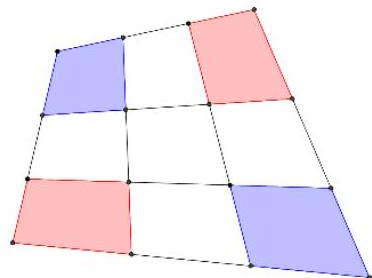
\includegraphics[max width=\textwidth, center]{2024_11_21_9bcf201a4fb59f89a03bg-1(2)}\\
części.
  \item Dany jest trójkąt \(A B C\). Punkt \(M\) jest środkiem tego łuku \(B C\) okręgu opisanego, do którego nie należy punkt \(A\). Udowodnij, że punkt \(I\) należący do odcinka \(A M\) jest środkiem okręgu wpisanego w trójkąt \(A B C\) wtedy i tylko wtedy, gdy \(M I=M B=M C\).
\end{enumerate}

\end{document}